\clearpage
\markboth{Problem 5}{Problem 5: Part 4}

\textbf{Problem Statement:} Implement and analyze the Ridders' method for solving the equation $f(x) = 0$. For guidance, you might wish to read the Wikipedia page on the Ridders' method. Also feel free to consult other sources.

\subsection*{Brief Description of the method}

Given the initial bracketing interval $[x_0, x_2]$, containing \textbf{one} solution, and such that $f(x_0)$ and $f(x_2)$ have opposite signs, compute the midpoint $x_1 = (x_0 + x_2)/2$. Then define a new function $h(x) = f(x)e^{ax}$. Find the parameter $a$ that ensures $h(x_1) = \frac{1}{2}(h(x_0) + h(x_2))$. Then define $x_3$ as the $x$-intercept of the line passing through $(x_0, h(x_0))$ and $(x_2, h(x_2))$. Use $x_3$ as one of the endpoints of the next interval bracketing the solution. The other endpoint is $x_1$ if $f(x_1)f(x_3) < 0$. Otherwise, choose either $x_0$ or $x_2$ based on the requirement that the sign of $f(x)$ at the chosen point must be opposite to the sign of $f(x_3)$. Continue until the desired accuracy is reached.

\subsection*{Part 4}
\addcontentsline{toc}{subsection}{Problem 5.4}

Numerically, compare the convergence rate of both algorithms. Discuss the results. What is the approximate order of convergence for the Ridders' algorithm?

\noindent\rule{\textwidth}{0.4pt}

\vspace{1em}

\textbf{Solution:}

\subsubsection*{Need for a Wider Interval}

The interval $[\text{-}0.8,\,\text{-}0.6]$ from Part 3 is too small for convergence analysis---Ridders' method converges in just 1 iteration, preventing observation of convergence behavior. To properly compare both algorithms, I use the wider interval $[\text{-}100,\,100]$ with tolerances $\epsilon = \delta = 10^{-12}$. This generates enough iterations to compute meaningful convergence orders and demonstrates robustness when starting far from the root. The MVT condition is satisfied: $f(\text{-}100) \cdot f(100) < 0$.

\subsubsection*{Convergence Analysis Results}

\paragraph{Ridders' Method}

Ridders' method converged in \textbf{12 iterations} to machine precision ($\approx 10^{-16}$), as shown in \Cref{fig:ridders-output,fig:ridders-convergence-trajectory}.

\begin{figure}[h!]
    \centering
    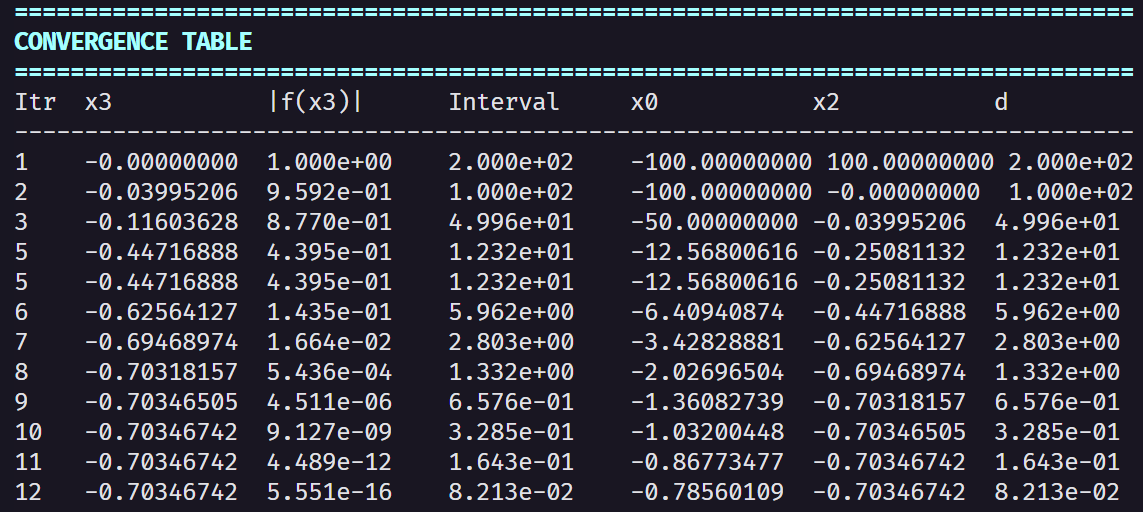
\includegraphics[width=\textwidth]{figures/p05-4-ridders-method-output-on-ex-x2.png}
    \caption{Ridders' method terminal output: 12 iterations to convergence.}
    \label{fig:ridders-output}
\end{figure}

\begin{figure}[h!]
    \centering
    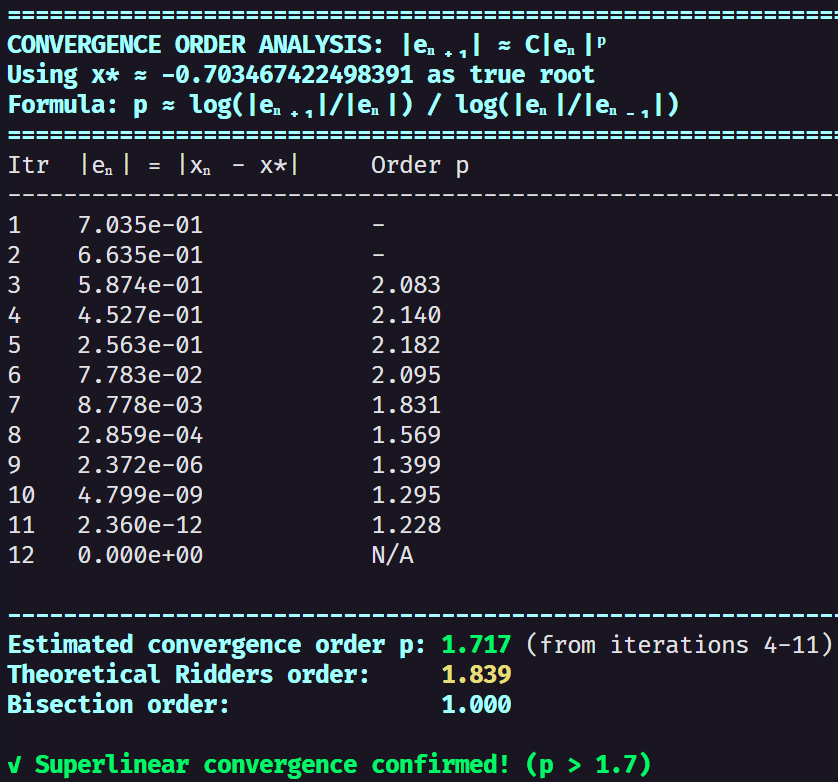
\includegraphics[width=0.95\textwidth]{figures/p05-4-ridders-method-convergence-table-on-ex-x2.png}
    \caption{Ridders' convergence trajectory table: rapid decrease in interval size demonstrates superlinear convergence.}
    \label{fig:ridders-convergence-trajectory}
\end{figure}

\clearpage

\paragraph{Bisection Method}

Bisection required \textbf{47 iterations}---almost 4$\times$ more than Ridders---to achieve similar accuracy, as shown in \Cref{fig:bisection-output-extended,fig:bisection-convergence-trajectory}.

\begin{figure}[h!]
    \centering
    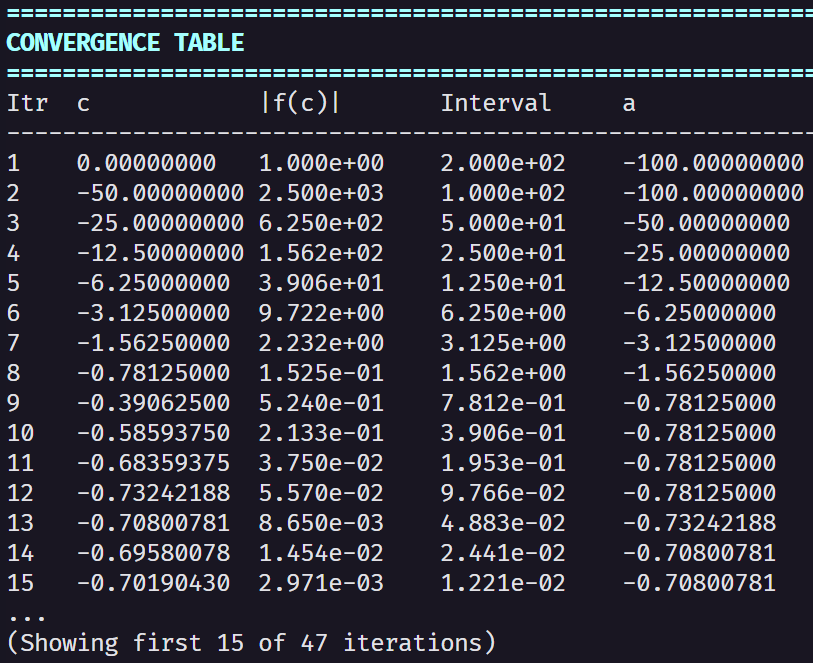
\includegraphics[width=\textwidth]{figures/p05-4-bisection-method-output-on-ex-x2.png}
    \caption{Bisection method terminal output: 47 iterations to convergence.}
    \label{fig:bisection-output-extended}
\end{figure}

\begin{figure}[h!]
    \centering
    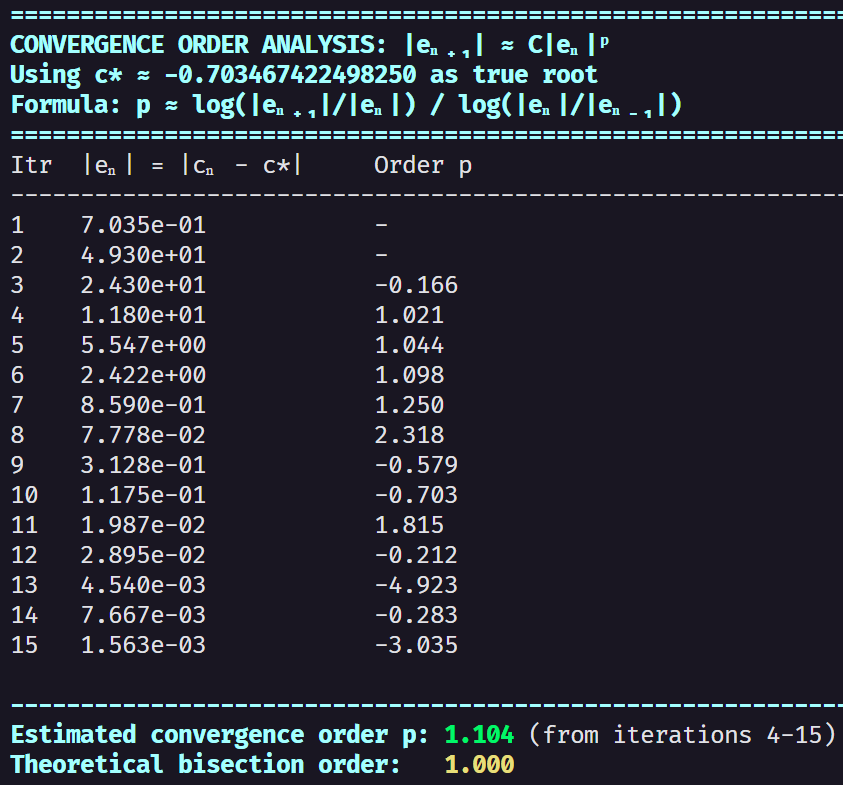
\includegraphics[width=0.95\textwidth]{figures/p05-4-bisection-method-convergence-table-on-ex-x2.png}
    \caption{Bisection convergence trajectory table (first 15 of 47 iterations): standard error analysis doesn't quite capture any particular convergence behavior, which is why typically bisection's convergence is described as linear with $|e_{n+1}| = \frac{1}{2}|e_n|$ based on interval halving.}
    \label{fig:bisection-convergence-trajectory}
\end{figure}

\clearpage

\subsubsection*{Convergence Order Analysis}

I computed the convergence order using: $p \approx \frac{\log(|e_{n+1}|/|e_n|)}{\log(|e_n|/|e_{n-1}|)}$ where $e_n = |x_n - x^*|$.

\paragraph{Ridders' Method:} $p \approx 1.717$ (iterations 4--11), close to theoretical $p = 1.839$. This confirms \textbf{superlinear convergence}.

\paragraph{Bisection Method:} $p \approx 1.104$ (iterations 4--15), close to theoretical $p = 1.0$. This confirms \textbf{linear convergence}. 

\textbf{Note:} Bisection's order is typically expressed as $|e_{n+1}| = \frac{1}{2}|e_n|$ (interval halving), but for direct comparison with Ridders, I used the same formula above.

\subsubsection*{Conclusions}

\begin{itemize}
    \item \textbf{Efficiency:} Ridders requires 12 iterations vs. bisection's 47 (4$\times$ faster) for tolerance $10^{-12}$
    \item \textbf{Convergence:} Ridders' $p \approx 1.717$ (superlinear) vs. bisection's $p \approx 1.0$ (linear)
    \item \textbf{Robustness:} Both converged successfully from the wide interval $[\text{-}100,\,100]$
\end{itemize}

Ridders' method is substantially more efficient than bisection, making it the preferred choice when function evaluations are not prohibitively expensive.

\vspace{2em}
\noindent\rule{\textwidth}{0.4pt}
